\chapter{\xlabel{data_files}SCUBA-2 Diagnostic Tools}
\label{sec:raw}

This chapter describes a number of procedures visualising and
assessing the quality of raw data files.  These steps need not be part
of your data reduction process and do not concern the iterative
map-maker.

However, there are reasons you may wish to examine your raw data in
greater depth. The most likely motivation is unusual result from  your
reduction such as higher than expected noise, artefacts in your map,
or inconsistent noise across multiple tiles.  This chapter will help
you get to the bottom of many of these issues.


\section{\xlabel{concat}Concatenate \& apply a flat-field}
\label{sec:concat}

Since SCUBA-2 data for a given sub-array are broken into multiple
30-second scans by the data acquisition (DA) system, it is useful to
concatenate the data into a single file. The \smurf\ task \concat\ can
be used for this operation. The example below combines all of the
files associated with Observation 8 for the s8a array into a single
file called \file{s8a20120725\_0008\_con}.

\begin{terminalv}
% sc2concat s8a20120725_0008\*.sdf s8a20120725_0008_con
\end{terminalv}

\task{sc2concat} will automatically filter out any dark or flat-field
observations, so that the concatenated file contains only the science
data. Be careful when concatenating a very long observation since the
output file may be too large to reasonably handle. Fifteen-minute
chunks (30 files) should be sufficient.

\task{sc2concat} applies the flat-field by default (although it can be
disabled using the \param{noflat} option on the command-line).

The flat-field can also be applied manually using the \flatfield\
command.

\begin{terminalv}
% flatfield 's8a20120701_0008*.sdf' '*_flat'
\end{terminalv}
Here, the output will be a flat-fielded version of each science scan
in Observation 8; the file names will be the original input
names with \_flat appended to them.

As a rule of thumb, you should apply the flat-field to your data
before examining it.


\begin{tip}
You do not need to apply the flat-field prior to reducing your
data with the map-maker.
\end{tip}

\section{\xlabel{header}Headers and file structure}
\label{sec:fitsheader}

There are two \Kappa\ tasks which are extremely useful for examining
your data: \fitslist\ and \ndftrace, which can be used to view the
FITS headers and dimensions of the data.


\begin{aligndesc}
\item[\textbf{\task{fitslist}:}] This lists the FITS header
  information for any file (raw or reduced). This extensive list
  includes dates \& times, source name, scan type, pattern and
  velocity, size of the map, exposure time, start and end elevation,
  opacity, and the temperature of the instrument. An example is given
  below:
\begin{terminalv}
% fitslist s8a20120720_00030_000\*.sdf | grep SEQ_TYPE
\end{terminalv}

If you already know the name of the parameter you want to view you can
use the \fitsval\ command instead, e.g.%\\
\begin{terminalv}
% fitsval file.sdf TAU225ST
\end{terminalv}

\item[\textbf{\task{ndftrace}:}] \task{ndftrace} displays the
  attributes of the data structure. This will tell you the units of
  the data, pixel bounds, dimensions, world coordinate bounds and
  attributes, and axis assignations.
\begin{terminalv}
% ndftrace file.sdf fullframe
\end{terminalv}

\end{aligndesc}


Full details of these commands can be found in the
\xref{\textsc{Kappa} manual}{sun95}{}.

\begin{figure}[ht!]
\begin{center}
\begin{fmpage}{0.95\linewidth}
\textbf{Topcat Example}
\minipageclear
\vspace{0.5cm}

\begin{minipage}[c]{0.6\linewidth}

\begin{terminalv}
% topcat -f tst 20120720_30.tst
\end{terminalv}
\end{minipage}
\hspace{0.3cm}
\begin{minipage}[c]{0.32\linewidth}
Load the tst file generated by \task{jcmtstate2cat} into \topcat.
\end{minipage}
\minipageclear

\vspace{0.5cm}

\begin{minipage}[c]{0.6\linewidth}
\begin{center}
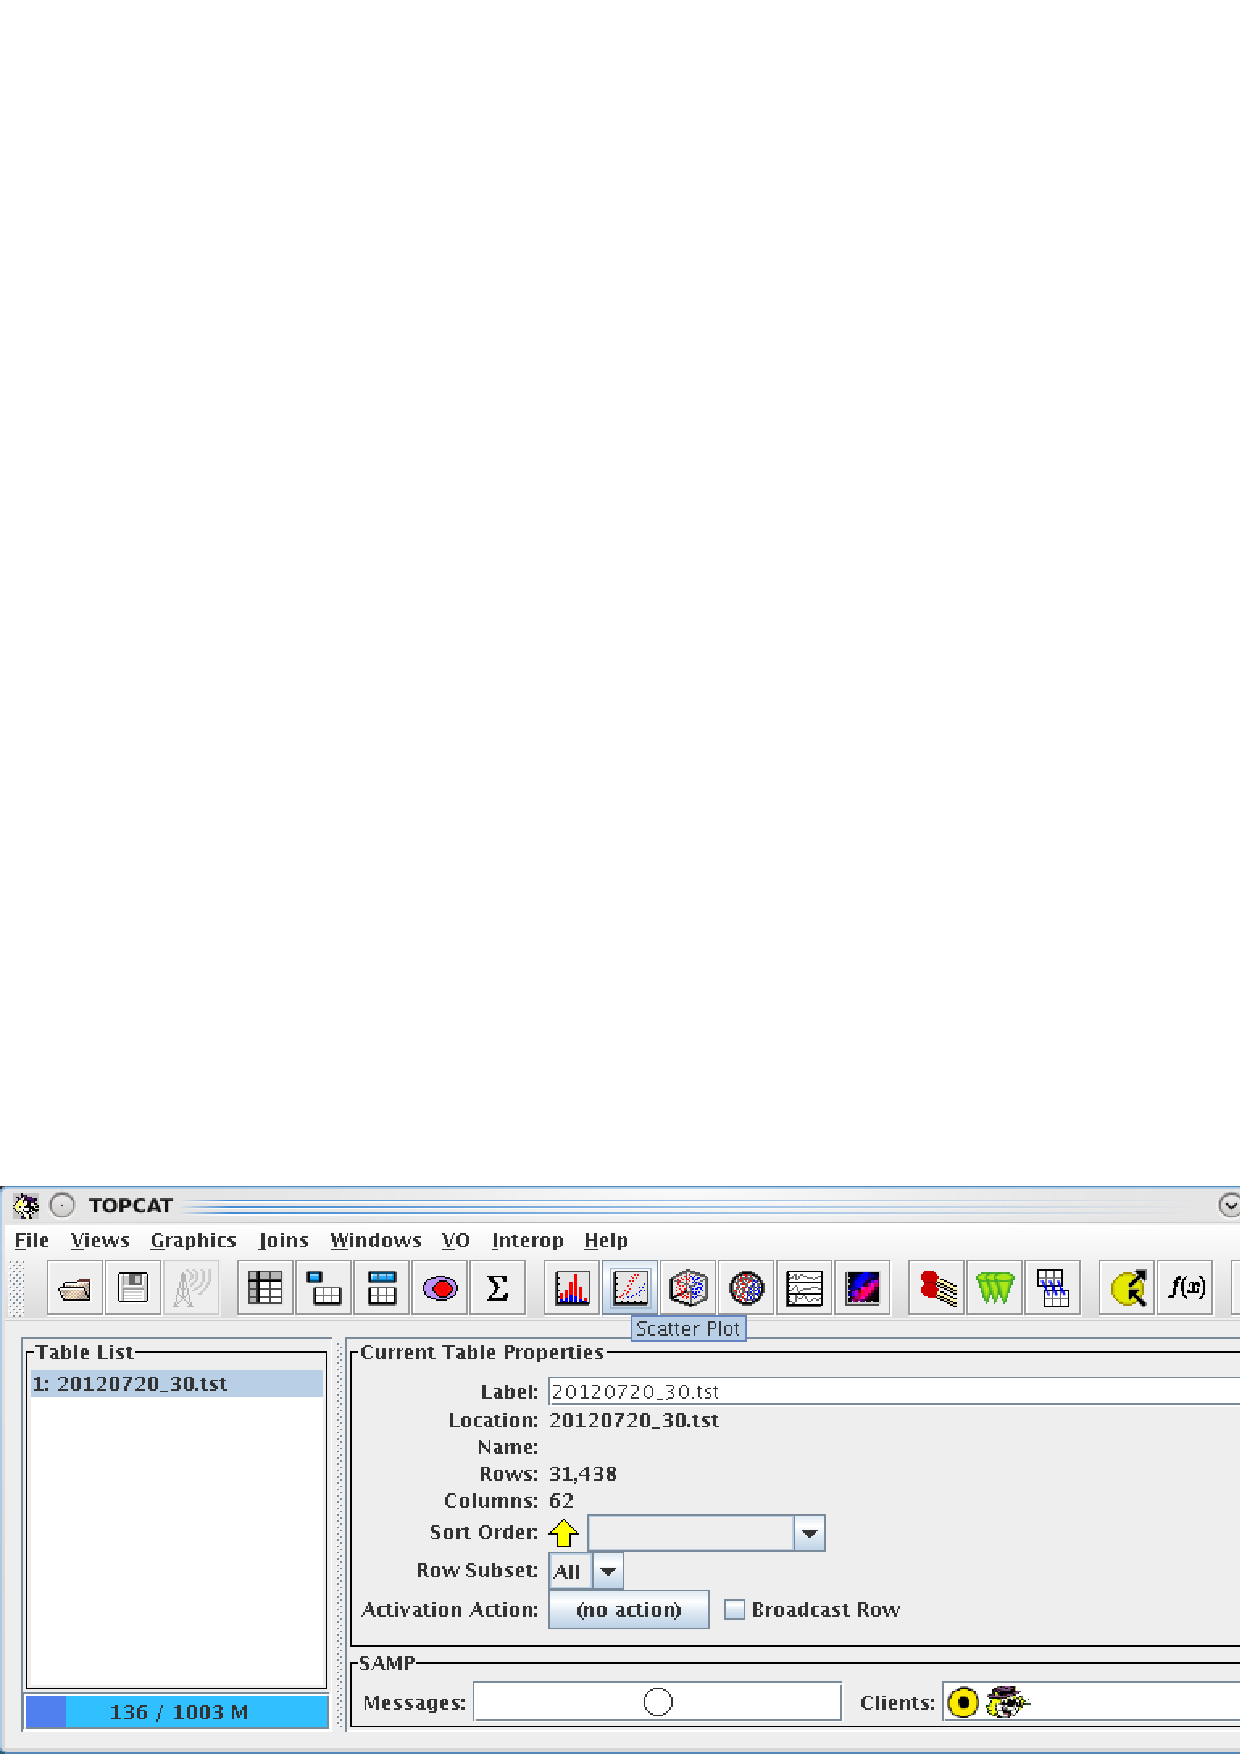
\includegraphics[width=0.95\textwidth]{sc21_topcat1}
\end{center}
\end{minipage}
\hspace{0.3cm}
\begin{minipage}[c]{0.32\linewidth}
In \topcat\ select the scatter plot option
from the menu bar across the top of the window.
\end{minipage}
\minipageclear
\vspace{0.5cm}

\begin{minipage}[c]{0.6\linewidth}
\begin{center}
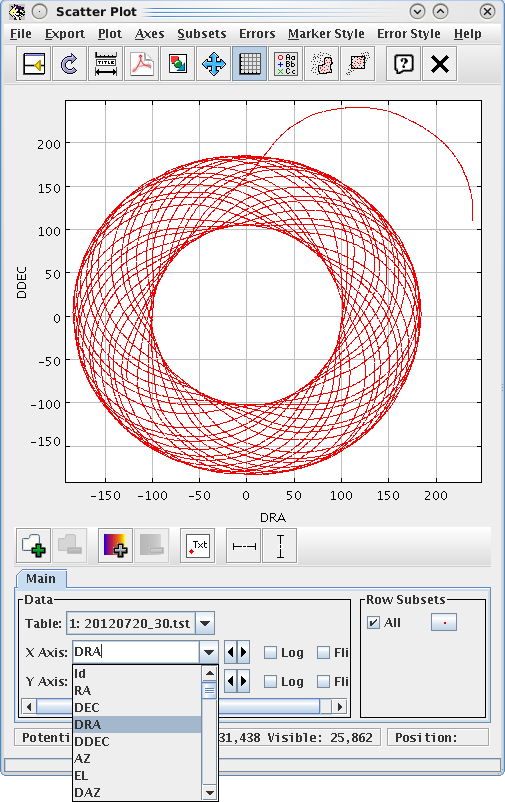
\includegraphics[width=0.75\textwidth]{sc21_topcat2}
\end{center}
\vspace{0.2cm}
\end{minipage}
\hspace{0.3cm}
\begin{minipage}[c]{0.32\linewidth}
With the scatter plot displayed you can adjust the $X$-axis and
$Y$-axis values to DRA and DDEC respectively to display the scan pattern.
If you are interested in seeing how any of the variables change over time,
select the the $X$ Axis to be either Id or RTS\_NUM.
\end{minipage}
\minipageclear

\end{fmpage}
\end{center}
\caption[Displaying the scan pattern with \topcat] { \small \topcat\
  example demonstrating how to display the scan pattern for an
  observation.  }
\label{fig:topcat}
\end{figure}


\section{\xlabel{scan_pat}Displaying scan patterns}
\label{sec:scan}

The movement of the telescope throughout a scan (as well as other
state information) is stored in the \texttt{MORE.SMURF.JCMTSTATE}
extension of a data file. The \smurf\ task \jcmtstate\ converts this
information into a simple ASCII tab-separated table.

\begin{terminalv}
% jcmtstate2cat s8a20120701_00008_*.sdf > state.tst
\end{terminalv}

Multiple files can be supplied to the command using standard shell
wild cards. If you have already concatenated your data you can simply
input the single concatenated file. It may be useful to view the scan
pattern for your observation, particularly for maps taken at high
elevations, to ensure the pattern completed successfully.


\begin{tip}
  Follow the \task{jcmtstate} command with \texttt{-h} to find out
  more information.
\end{tip}


This catalogue can be loaded into \topcat\ for plotting, making sure
to specify the TST format during loading.

\begin{terminalv}
% topcat -f tst state.tst
\end{terminalv}

Example of scan patterns displayed with \topcat\ can be seen in
\cref{Figure}{fig:scan}{telescope tracks}. Detailed instructions on
how to display the scan pattern for your observation are given in
\cref{Figure}{fig:topcat}{box below}.  All of the time-varying header
values are available for plotting. Other values include the azimuth
and elevation offsets (DAZ \& DEL), the WVM and 225\,GHz opacity
values, and the instrument temperatures (e.g.  SC2\_FPUTEMP gives the
temperature of the focal plane).

Due to extreme accelerations at ``turn-around'' points of a scan
pattern (especially for \textsc{pong}s), the telescope finds it hard
to follow the proscribed scan patterns at high elevations. To mitigate
this we try to avoid observing any sources above 70$^\circ$ elevation.
If the \fitslist\ keywords \param{ELSTART} and \param{ELEND}
indicate that your map was taken at high elevation you may consider
checking the success of the scan pattern. If you find your observation
has failed to follow the demanded scan pattern don't worry, the data are
likely to still be useful. This is especially true for \textsc{daisy}
maps where the high exposure-time central region is usually
unaffected.

\section{\xlabel{display_cube}Displaying time-series data}
\label{sec:gaiacube}

Use the \starlink\ application \textsc{Gaia} to visualise the
bolometer time-series data (or indeed \emph{any} SCUBA-2 data
file). This is initiated simply typing \texttt{gaia} into a terminal.

\begin{terminalv}
% gaia s8a20120725_00058_con.sdf
\end{terminalv}

Loading a file in \textsc{Gaia} produces two windows. The main window
(see \cref{Figure}{fig:gaia_main}{upper graphic}) shows a map of
bolometer values at a given point in time. The time slice displayed
may be changed by scrolling through the time axis. This is done in the
second window entitled \gaiathing{Display image sections of a
  cube}. The \gaiathing{Index of plane} slider towards the top of this
window may be moved to display different time slices in the main
window.

\starfig{sc21_gaia1}{[b]}{width=\linewidth}{fig:gaia_main}{
  Raw data displayed in the main \gaia\ window}{
  Initial \gaia\ windows displayed upon loading a data cube.
  The main window in the left shows a map of bolometer values at a fixed
  sample in time. You may have to zoom in multiple times by clicking the
  \gaiathing{Z} icon. On the right-hand side, the
  \gaiathing{Display image sections of a cube}
  dialogue enables you to navigate the time axis.
}

A third window will appear when you click on a bolometer---the
\gaiathing{Spectral plot} (see \cref{Figure}{fig:gaia_spec}{lower graphic}).
This shows an automatically scaled plot of the raw time stream of data for
that given bolometer. It will be overridden when you click on a different
bolometer.

\starfig{sc21_gaia2}{[t]}{width=0.8\linewidth}{fig:gaia_spec}{ \gaia\
  spectral plot window}{ The \gaiathing{Spectral plot} window displays
  the time-varying signal. This window appears automatically when a
  bolometer is clicked in the main window.  The vertical red line
  indicates the time slice that is currently selected in the
  \gaiathing{Display image sections of a cube} dialogue---this can be
  dragged across the spectrum to scroll through the time-slices.  }

A second way to scroll through the time axis is to click and drag the
vertical red bar on the \gaiathing{Spectral plot} window. As you do
so, the array shown in the main window will automatically update.

To highlight small variations between bolometers you will need to
change the auto cut and (depending on your preference) the colour
scheme---both are controlled by buttons on the sidebar.

See the \xref{\textsc{Gaia} manual}{sun214}{} for full
details.\footnote{\url{http://www.starlink.ac.uk/docs/sun214.htx/sun214.html}}


\section{\xlabel{regrid_map}Regridding data into a map}
\label{sec:regrid}

Any raw time-series data can be quickly regridded into sky frame
coordinates using the \smurf\ \makemap\ task in rebin mode. This
involves no processing of the data. The following command produces a
map from the raw concatenated data; unlike the iterative mode of
\task{makemap} described in the next chapter, no configuration file is
required.

\begin{terminalv}
% makemap s8a20120725_00058_con.sdf crl2688_sky method=rebin
\end{terminalv}

The output map here is called \file{crl2688\_sky.sdf} and is shown in
\cref{Figure}{fig:regrid}{the figure below}.  The pixel scale is left
at the default values of 2\,arcsec on a side at 450$\mu$m and
4\,arcsec at 850$\mu$m (although this can be changed using the
\texttt{pixsize=}$x$ option on the command-line, where $x$ is in
arcsec).

\starfig{sc21_crl2688_regrid}{[b!]}{width=0.65\linewidth}{fig:regrid}{
  The regridded map of CRL~2688 displayed with \gaia.}{ The regridded
  map of CRL~2688 with the s8a sub-array displayed with \gaia.  }

\begin{tip}
  If you do not include \param{method=rebin}, the map-maker will
  default to \param{method=iterate}.
\end{tip}


\section{\xlabel{clean}Notes on cleaning your data}
\label{sec:clean}

Cleaning raw data is an essential first step towards making a quality
final map. The map-maker performs all of these cleaning steps during
the pre-processing stage. The commands for manually cleaning your data
are given in \cref{Appendix}{app:clean}{Cleaning the raw data}.  You
can also check out the SMURF SRO
Cookbook{\footnote{\url{http://www.starlink.ac.uk/docs/sc19.htx/sc19.html}}}
which goes into great depth on the data cleaning options.


\section{\xlabel{calcnoise}Checking the array performance}
\label{sec:calcnoise}

The on-sky performance of the array can be assessed using the \smurf\
command \calcnoise. Rather than give an absolute measure,
\task{calcnoise} should be used as an indicator of array performance
and stability.  \task{calcnoise} cleans the data then calculates the
white noise on the array (between 2 and 10\,Hz by default).
\begin{terminalv}
% calcnoise s8a20110720_00030\*.sdf s8a_noise power=!
\end{terminalv}
It will prompt for a configuration file to describe the cleaning
steps. The default is the supplied \file{dimmconfig\_calcnoise.lis}.
Two noise measurements are reported in the terminal: the `Effective
noise' and the `Effective NEP'.

An output file is created for each sub-array with the NEP map stored
in the \texttt{.MORE.SMURF.NEP} extension.

If you have a bright source in the field this will contaminate the
signal. In this case you should examine the \model{NOI} model from the
map-maker instead---see \cref{Section}{sec:models}{The individual
  models} for a description and \cref{Section}{sec:export}{Exporting
  individual models} for details on how to examine it.

\section{\xlabel{export}Exporting individual models}
\label{sec:export}

By default, the final values of the models fitted by the map-maker are
\emph{not} written out. However, this can be changed by setting
\xparam{EXPORTNDF}{exportndf} in the configuration file to the list of models
that you wish to view.
%\vspace{0cm}

\begin{terminalv}
exportndf = (com,gai,ast,flt,res,noi,qua)
\end{terminalv}

In addition to the models listed in \cref{Section}{sec:models}{The
individual models}, you can request \model{RES} in order to export the
\model{RES} model --- the residual signal remaining after
the other models have been removed.  If \model{NOI} (the estimate of
the bolometer noise levels) is exported, it is stored as the VARIANCE
component of the \model{RES} model; thus, export of \model{RES} is implied
if \model{NOI} is specified.

The \texttt{exportndf} parameter will write out the requested models
as NDF files with names based on the first input file that went into
the maps for each sub-array. This is first suffixed by \texttt{con},
indicating that several data files may have been concatenated
together. The three-letter code for each model is then appended to the
filename (such as \file{s8a20120720\_00030\_0003\_con\_com.sdf},
\file{s8a20120720\_00030\_0003\_con\_flt.sdf},
\file{s8a20120720\_00030\_0003\_con\_res.sdf})\footnote{The filename
shows the third sub-scan of Observation 30 since this is the first science
file that is encountered (see \cref{Chapter}{sec:raw}{Handling Raw
SCUBA-2 Data}).~} The variance and quality for the data are stored as
the VARIANCE and QUALITY components within the residual file NDF.

\begin{tip}
  These exported model components are 3-dimensional arrays with axes \texttt{
  (bolometer column, bolometer row, time slice index)}, and so can be viewed
  using the cube visualisation facilities within \gaia\ (see \gaiasun).
\end{tip}



